\chapter{Evaluation}

\section{Measures of Success}

The success of the project can be measured by comparing the project results with objectives. We will also review the design choices in constructing the tool. The review will highlight the practical outcomes from using argumentation to explain scheduling.
\linespace
Arguably, the most important outcome of this project is that the tool is functionality correct. This means the tool is required to explain schedules for feasibility, efficiency and satisfaction with respect to user decisions.
\linespace
One objective is to implement an accessible tool. To measure accessibility, we can refer to the tractability complexity from explanations. The length of explanations either in the number of words or characters may be correlated with understandability. Alternatively, we can conduct a survey targetted towards potential users. Because the understandability of explanations are difficult to measure, we will attempt to quantity this using multiple choice questions. To carefully evaluate explanations, one would need to refer to cognitive science, which is beyond the scope of this project. In addition, we can measure performance to reflect responsiveness and scalability of the tool. This may be achieved by using profiling utilities to measure performance metrics such as time to generate explanations and memory consumption.
\linespace
We can also use the survey to ask how well our tool performs with respect to applicability and knowledge transfer. We can also infer the practical limitations from the tool to measure the applicability.

\section{Theoretical Results}

At the end of the project, we aim to present extensions of argumentation with scheduling We will explain the practicability of using argumentation Such details are open-ended.

\section{Practical Results} 

I will be able to demonstrate the tool, and its functionality. This will be reflected in the report through a user documentation guide.

\subsection{Full vs. Partial Precomputation}

\begin{figure}[H]
	\centering
	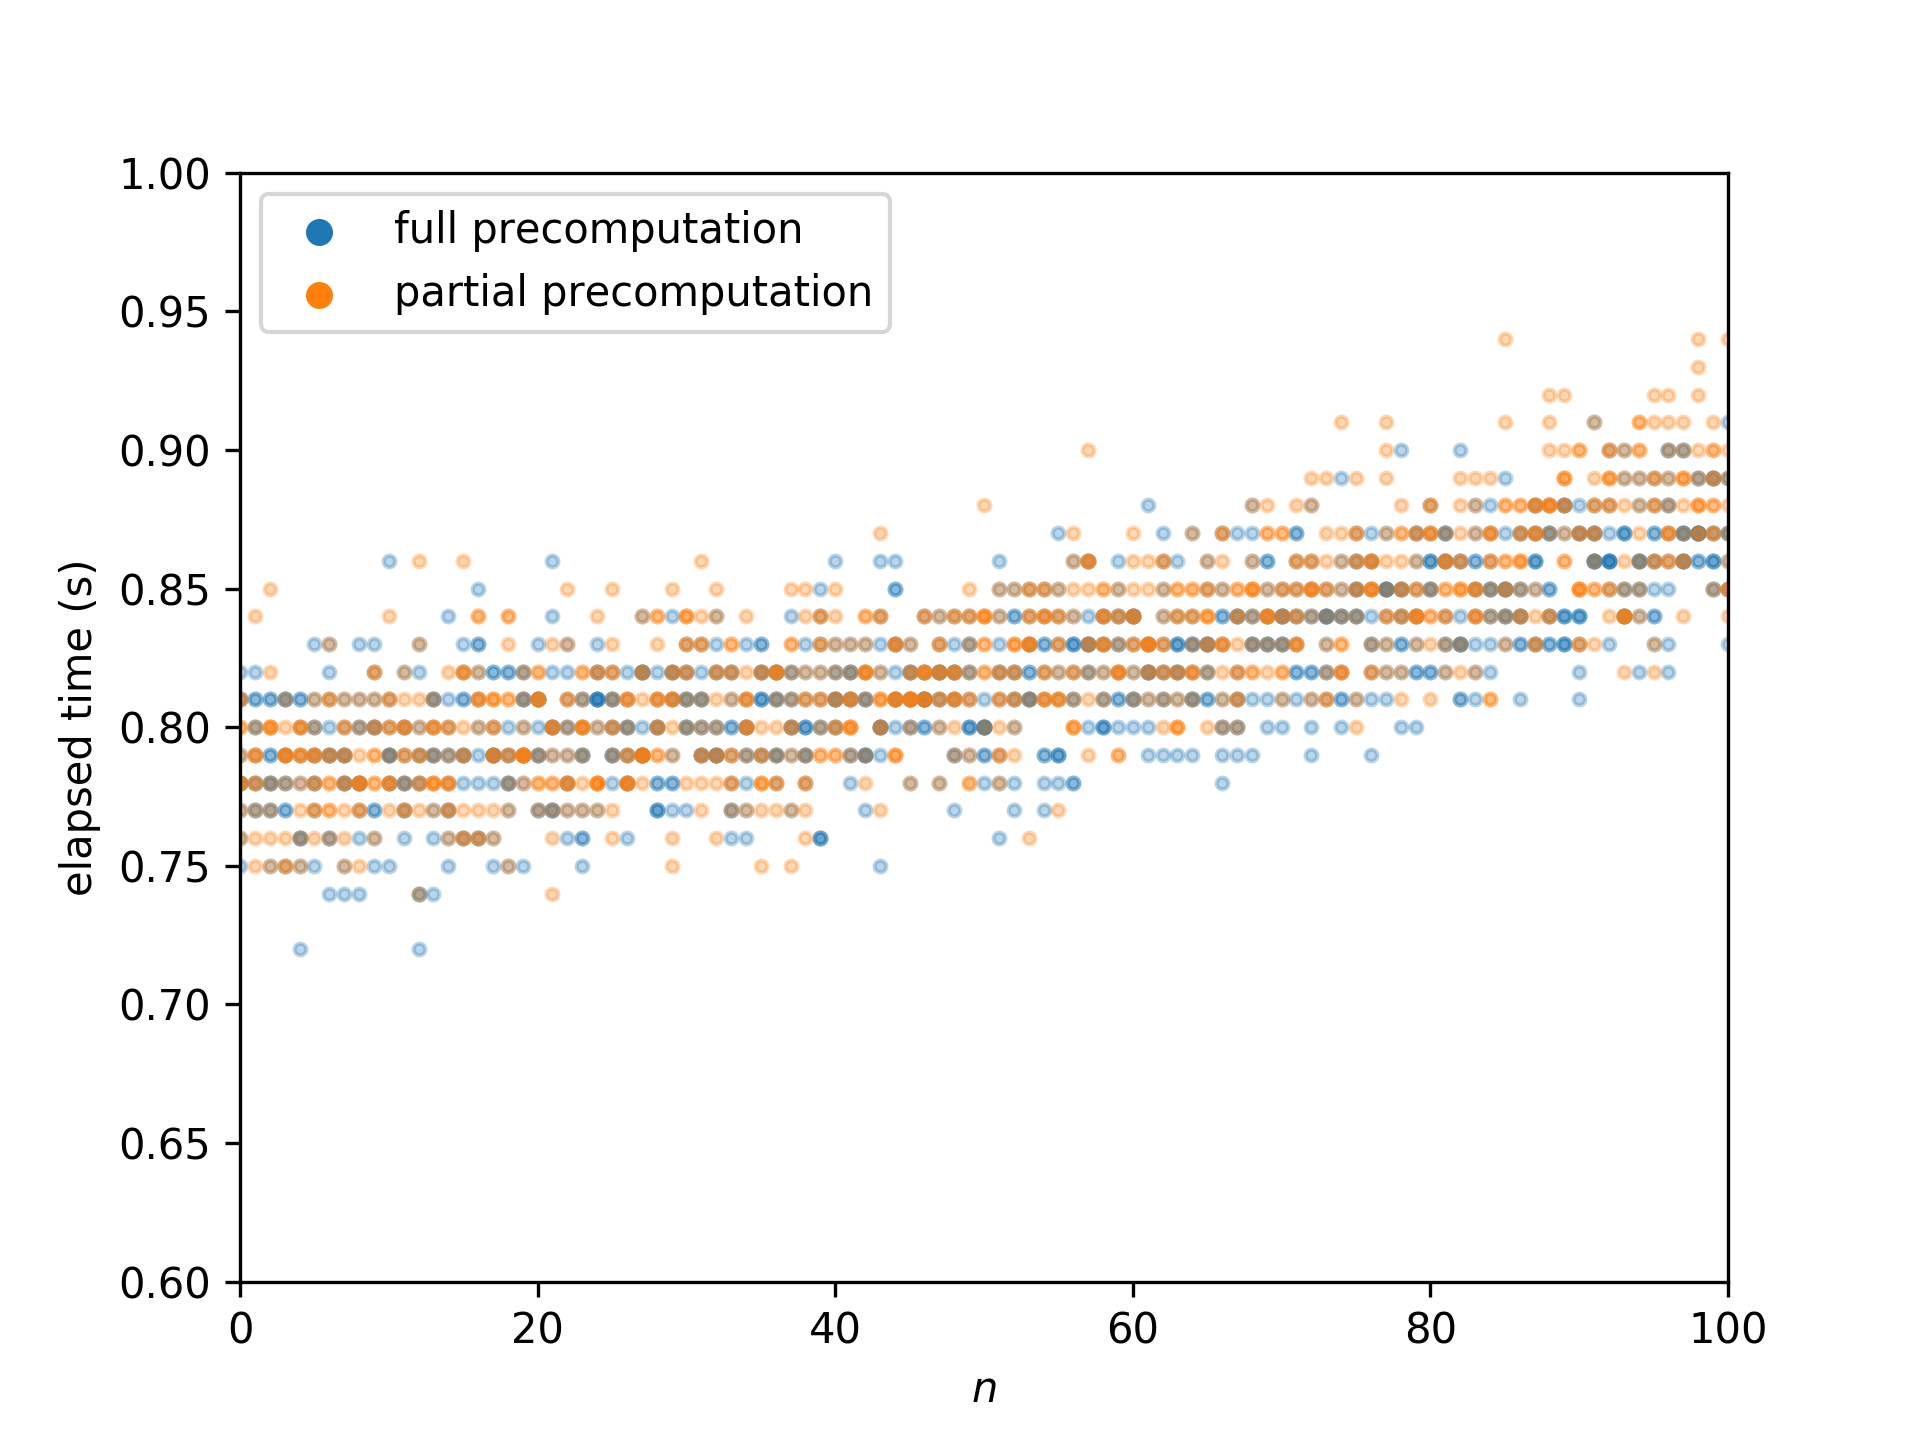
\includegraphics[scale=0.6]{figures/precomputation_cpu_small}
	\caption{CPU elapsed time comparison for small number of jobs where $m=10$}
\end{figure}

\begin{figure}[H]
	\centering
	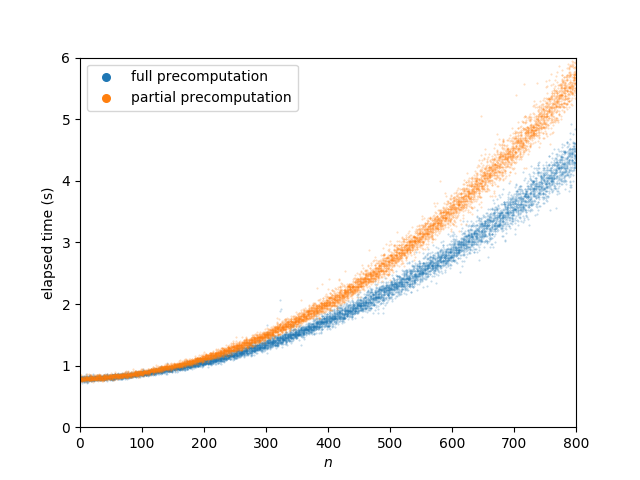
\includegraphics[scale=0.6]{figures/precomputation_cpu_big}
	\caption{CPU elapsed time comparison for large number of jobs where $m=10$}
\end{figure}

\begin{figure}[H]
	\centering
	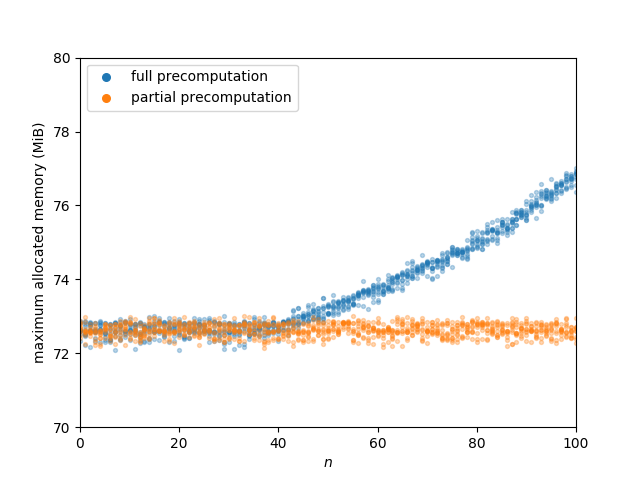
\includegraphics[scale=0.6]{figures/precomputation_memory_small}
	\caption{Maximum allocated memory comparison for large number of jobs where $m=10$}
\end{figure}

\begin{figure}[H]
	\centering
	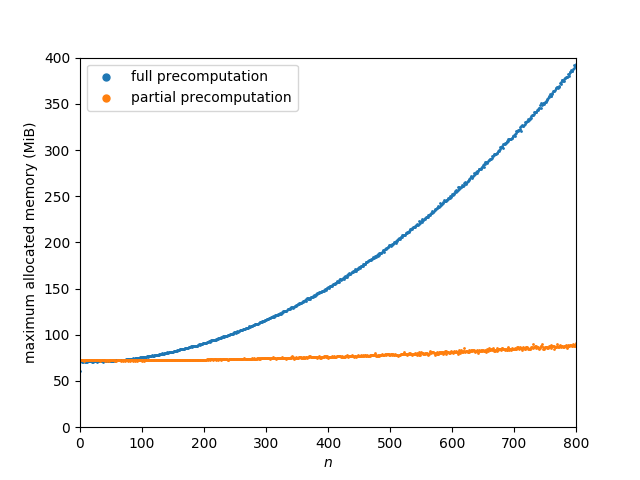
\includegraphics[scale=0.6]{figures/precomputation_memory_big}
	\caption{Maximum allocated memory comparison for large number of jobs where $m=10$}
\end{figure}